\documentclass[11pt]{article}
\usepackage[T1]{fontenc}
\usepackage[utf8]{inputenc}
\usepackage[margin=1in]{geometry}
\usepackage{amsmath, amssymb}
\usepackage{booktabs}
\usepackage{graphicx}
\usepackage{caption}
\usepackage[hidelinks]{hyperref}
\usepackage{setspace}
\setstretch{1.08}
\setlength{\parskip}{0.5em}

\title{Sensitivity-Guided Bit Allocation for Low-Bit Weight Quantization of Qwen3.5-4B}
\author{Project report}
\date{October 2026}

\begin{document}
\maketitle

\begin{abstract}
We measure how sensitive each decoder linear group of Qwen3.5-4B is to symmetric per-channel weight quantization at 8, 6, 4, 3, and 2 bits. Sensitivity is the change in Wikitext-2 perplexity when one group is quantized and all others stay at full precision. The model has 64 such groups (32 layers, each split into a mixer and an MLP part), covering 3.57 billion weights. A greedy allocator then assigns widths under average-bit budgets from 3 to 6. We compare it with uniform and random assignments on held-out test perplexity. Among allocations that stay within the budget, greedy beats uniform at every budget. It is about 2 percent better at 6 and 4 bits, and 2.4 times better at 3 bits, where all methods are unusable. At fractional budgets, a log-linear interpolation of the uniform curve is 3 to 13 percent higher than greedy between 4 and 6 bits, and 3.8 times higher at 3.5 bits. It lies far below random assignments throughout. The additive sensitivity model ranks configurations well (Spearman 0.96 over unique points), but it underestimates perplexity by a factor that grows as the budget falls. One layer dominates the 2-bit error. Single-group measurements are noisy at the scale of the effects near 4 bits, so we report the measurement limits alongside the results.
\end{abstract}

\section{Introduction}

Weight quantization reduces the memory and bandwidth a language model needs at inference time. The simplest scheme gives every matrix the same width, but matrices differ in how much error they can absorb. Mixed-precision methods therefore choose a width per matrix under a total budget. The question for such a method is which matrices deserve the extra bits.

This report measures that structure for Qwen3.5-4B. We quantize one decoder group at a time, record the perplexity change, and use these measurements to allocate bits under average-bit budgets. We then compare the allocations on a separate test split. The study answers four questions: how sensitivity varies across layers and between mixer and MLP parts; whether sensitivity-guided allocation beats uniform and random assignments; how well an additive model of per-group costs predicts the measured perplexity of a full allocation; and how much measurement noise limits the conclusions.

The contributions are a per-group sensitivity table over five widths, a comparison of three allocation strategies at six budgets evaluated on the same data, an empirical check of the additive model, and a documented account of the measurement limits.

\section{Setup}

\subsection{Model and data}

The model is Qwen/Qwen3.5-4B in bfloat16. Its 32 decoder layers follow a 3:1 hybrid pattern: 24 layers use a linear-attention (DeltaNet) mixer, and 8 layers use full attention, at zero-indexed layers 3, 7, 11, \ldots, 31. The target set is every \texttt{nn.Linear} inside a decoder layer, excluding any vision path. This gives 248 modules: 152 in the mixer part and 96 in the MLP part. Together they hold 3{,}569{,}090{,}560 weights, which is 84.9 percent of all parameters. Embeddings, the output head, and normalization weights stay in full precision.

Sensitivity is measured on the first 16 non-overlapping windows of 2048 tokens from the Wikitext-2 raw training split, which gives 32{,}768 tokens. Test perplexity uses all 145 non-overlapping windows of the test split, which gives 296{,}960 tokens. The unquantized model scores 9.861 on the sensitivity windows and 9.584 on the test windows. Each evaluation runs the windows through the model in batches of four and computes next-token cross entropy over every predicted position.

\subsection{Quantizer}

The quantizer is symmetric and per output row, because a linear weight has shape (out, in) and each output row has its own range. For bit width $b$ let $q_{\max} = 2^{b-1} - 1$. Each row gets a scale $s_r$ that maps its largest magnitude to $q_{\max}$:
\begin{equation}
s_r = \frac{\max_j |W_{rj}|}{q_{\max}}, \qquad
\hat W_{rj} = s_r \,\mathrm{round}\!\left(\frac{W_{rj}}{s_r}\right).
\end{equation}
The intuition is simple. Each row is cut into an evenly spaced grid whose step is set by its largest weight, and every weight snaps to the nearest grid point. Because the scale comes from the row maximum, no weight falls outside the grid, so the clamp to $[-q_{\max}, q_{\max}]$ never activates. Each weight therefore moves by at most half a step:
\begin{equation}
|\hat W_{rj} - W_{rj}| \le \tfrac{1}{2} s_r.
\end{equation}
Rounding an already quantized row returns the same row, so the quantizer is idempotent. A runtime check in the code confirms the half-step bound and idempotence on a real model matrix, at 8 bits.

The width of the grid determines the error. Going from $b$ to $b+1$ bits roughly halves $s_r$. If the rounding error of a weight is spread evenly over one step, its mean squared error is about $s_r^2/12$. With $s_r \approx \max_j |W_{rj}|\, 2^{1-b}$, the error scales as $4^{-b}$, so each extra bit cuts the squared error by about a factor of four, or roughly 6 dB. This is an approximation. It is reasonable for $b \ge 3$, but at 2 bits the grid has only three points, and the largest weights dominate the error.

Each grid has $2q_{\max} + 1 = 2^b - 1$ levels, not $2^b$. Consequently, the 8-, 6-, 4-, 3-, and 2-bit grids have 255, 63, 15, 7, and 3 levels. The reported widths are nominal, and we keep that convention throughout.

\subsection{Bit accounting}

A budget is an average bit width over decoder linear weights. For unit $u$ with $n_u$ weights at width $b_u$, the average is
\begin{equation}
\bar b = \frac{\sum_u n_u b_u}{\sum_u n_u}, \qquad \sum_u n_u = N = 3{,}569{,}090{,}560.
\end{equation}
The average excludes the per-row scales. Each scale is one 16-bit value per output row, so the overhead is $16/d_{\mathrm{in}}$ bits per weight, where $d_{\mathrm{in}}$ is the input dimension. That is between 0.0017 and 0.0063 bits per weight for the input sizes in this model, so the exclusion does not change any conclusion. Expressed relative to bfloat16, a budget of $B$ bits is $B/16$ of the full-precision size. The unquantized baseline is recorded as eight bits in the results file, which is a placeholder and not a measured width.

\section{Method}

\subsection{Sensitivity measurement}

A unit is a group of linear modules that share a layer index and a part, either mixer or MLP. At each of the five widths, one unit is quantized while every other weight stays at full precision. Its cost is the change in perplexity on the sensitivity windows, measured against the unquantized baseline:
\begin{equation}
c_u(b) = \mathrm{PPL}_{\mathrm{sens}}(u \text{ at } b \text{ bits}) - \mathrm{PPL}_0.
\end{equation}
Weights are restored after each measurement, and the baseline is measured again after the grid to check for drift. In total, the grid has $64 \times 5 = 320$ entries.

\subsection{Allocation problem}

Choose a width $b_u$ from the set $\{8, 6, 4, 3, 2\}$ for each unit so that the total measured cost is small while the average width stays within the budget $B$:
\begin{equation}
\min_{b_u \in \{8,6,4,3,2\}} \sum_u c_u(b_u) \quad \text{subject to} \quad \sum_u n_u b_u \le B\, N.
\end{equation}
This is a multiple-choice knapsack problem with separable costs. We use a greedy heuristic rather than an exact solver, which keeps the procedure short and easy to trace.

\subsection{Greedy, uniform, and random allocations}

The greedy allocator starts every unit at 8 bits. At each step it considers, for every unit, the one-step downgrade to the next lower width $b'$. It scores each downgrade by its cost per weighted bit saved:
\begin{equation}
\rho_u = \frac{c_u(b') - c_u(b)}{n_u\,(b - b')},
\end{equation}
applies the downgrade with the smallest $\rho_u$, and repeats until the average width is within the budget. The intuition is that $\rho$ is a price for one weighted bit, and the greedy rule equalizes that price across units. When each unit's cost is convex in its width, this rule is optimal for the separable problem. The measured costs are not guaranteed to be convex, so the result is a heuristic.

The uniform allocator sets every unit to one width. For a budget $B$ that is not on the grid, we evaluate the largest width below it and the smallest width above it. When $B$ is itself a width, the two are identical, and the duplicate evaluation is omitted.

The random allocator starts every unit at 8 bits and repeatedly picks a unit uniformly at random among those above the minimum width, then lowers it by one step until the budget is met. We repeat this with seeds 0, 1, and 2.

Every allocation is applied to all units together, and both perplexities are measured on the full model. Weights are restored afterward, so each method starts from the unquantized model.

\subsection{Additive predictor}

If the cost of each unit is independent of the others, the predicted perplexity of an allocation is
\begin{equation}
\widehat{\mathrm{PPL}}(\{b_u\}) = \mathrm{PPL}_0 + \sum_u c_u(b_u).
\end{equation}
This predictor is computed for every allocation, including the uniform and random ones. Its agreement with the measured sensitivity perplexity tests whether the costs add. The predictor uses only the sensitivity table, so the test split plays no part in it.

\section{Results}

\subsection{Sensitivity structure}

Figure~\ref{fig:heatmap} shows the cost of each unit at each width. Values above 1.5 are shown at the top of the scale. Two patterns stand out. First, the cost rises sharply below 4 bits, and the median unit moves from about 0.03 at 4 bits to 0.12 at 3 bits and 0.46 at 2 bits. Second, the costs are highly skewed. At 8 bits the measured changes lie between $-0.016$ and $0.020$, with a standard deviation of 0.005. That spread is the noise floor of the measurement, because 8-bit quantization should change the model very little. Figure~\ref{fig:parts} shows the same data as medians over units, separately for the mixer and MLP parts. From 4 bits down, the MLP median is higher than the mixer median: 0.036 against 0.021 at 4 bits, and 0.171 against 0.101 at 3 bits. At 8 and 6 bits the two medians are indistinguishable from zero.

\begin{figure}[t]
\centering
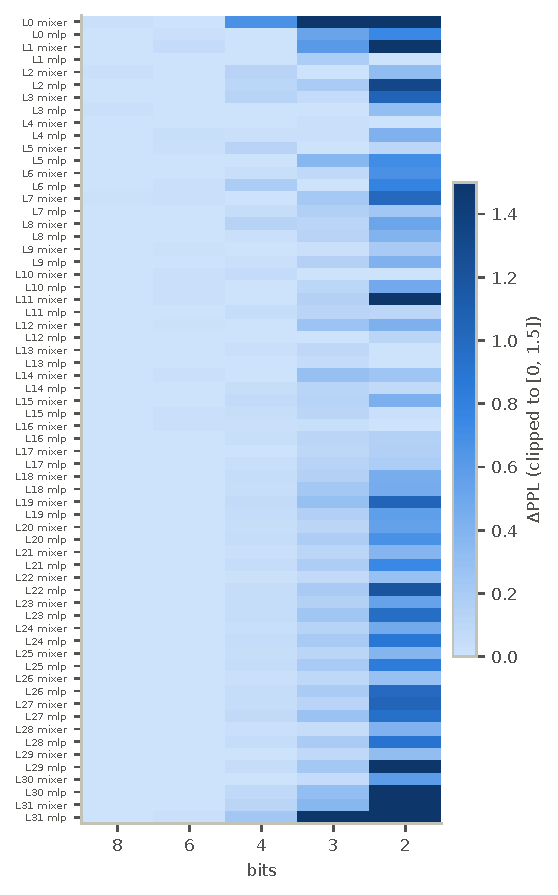
\includegraphics[height=0.55\textheight]{figures/fig1_sensitivity_heatmap.pdf}
\caption{Measured cost $c_u(b)$ for each unit (rows, ordered by layer, mixer before MLP) and width (columns). Values are clipped to $[0, 1.5]$ for display, so negative measurements appear at the bottom of the scale. The 2-bit cost of layer 0 mixer, 3{,}411, is saturated.}
\label{fig:heatmap}
\end{figure}

\begin{figure}[t]
\centering
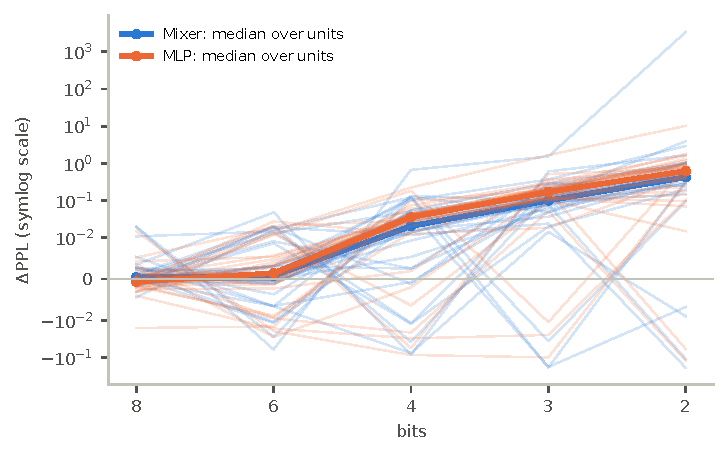
\includegraphics[width=0.85\textwidth]{figures/fig2_sensitivity_by_part.pdf}
\caption{Cost by width for every unit (thin lines) and the median over units within each part (thick lines). The vertical scale is symmetric-log, linear near zero and logarithmic above $10^{-2}$.}
\label{fig:parts}
\end{figure}

A few units dominate. Table~\ref{tab:outliers} lists the largest costs. Layer 0 mixer costs 0.67 at 4 bits, 1.54 at 3 bits, and 3{,}411 at 2 bits. At 2 bits it accounts for 98.6 percent of the summed cost over all units. Layer 31 MLP is the largest cost at 3 bits (1.67) and the second largest at 2 bits (10.2). The greedy allocator therefore keeps layer 0 mixer at 6 bits at every budget we tested.

\begin{table}[t]
\centering
\caption{Units with the largest measured cost at each low width.}
\label{tab:outliers}
\begin{tabular}{llrr}
\toprule
Bits & Unit & Parameters (M) & $\Delta$PPL \\
\midrule
4 & L0 mixer & 42.1 & 0.670 \\
4 & L31 mlp & 70.8 & 0.225 \\
4 & L6 mlp & 70.8 & 0.183 \\
\midrule
3 & L31 mlp & 70.8 & 1.669 \\
3 & L0 mixer & 42.1 & 1.536 \\
3 & L1 mixer & 42.1 & 0.609 \\
\midrule
2 & L0 mixer & 42.1 & 3411.489 \\
2 & L31 mlp & 70.8 & 10.232 \\
2 & L11 mixer & 36.7 & 3.936 \\
\bottomrule
\end{tabular}

\end{table}

Many costs are smaller than the noise. Across the 64 units, 41 show a width where the measured cost falls when the width is lowered. Of these, 16 have a fall greater than 0.05 perplexity, 9 have a fall greater than 0.1, and 4 have a fall greater than 0.2. Such values are not evidence that a unit prefers lower precision. They show that single-group differences near 0.1 are at the limit of what 16 windows can resolve.

The parameter counts identify the layer types. The eight full-attention layers have a mixer of 36.7 million weights each, and the 24 DeltaNet layers have mixers of 42.1 million weights each. All MLP units have 70.8 million weights. The parameter counts follow directly from the configured dimensions, and the layer type pattern is confirmed by the run log.

\subsection{Allocation quality}

Table~\ref{tab:main} gives test perplexity for each budget. Figure~\ref{fig:ppl} plots the same results against the average width. The greedy allocation reaches each budget with an average width within 0.02 bits of its target, and the uniform reference uses the nearest widths on either side.

\begin{table}[t]
\centering
\caption{Test perplexity by budget. Greedy uses the average width shown. Uniform uses the widths below and above the budget; the above row is omitted when the budget equals a width, since it is then the same allocation. The unquantized test perplexity is 9.58.}
\label{tab:main}
\begin{tabular}{rrrrrrrr}
\toprule
Budget $B$ & \multicolumn{2}{c}{Greedy} & \multicolumn{2}{c}{Uniform, $\lfloor B \rfloor$} & \multicolumn{2}{c}{Uniform, $\lceil B \rceil$} & Random median \\
 & bits & PPL & bits & PPL & bits & PPL & PPL \\
\midrule
6 & 5.99 & 9.39 & 6 & 9.62 & \multicolumn{2}{c}{omitted} & 14.26 \\
5 & 4.98 & 9.96 & 4 & 12.82 & 6 & 9.62 & 51.84 \\
4.5 & 4.50 & 10.53 & 4 & 12.82 & 6 & 9.62 & 148.17 \\
4 & 3.99 & 12.58 & 4 & 12.82 & \multicolumn{2}{c}{omitted} & 822.18 \\
3.5 & 3.49 & 33.46 & 3 & 1,128 & 4 & 12.82 & 85,170 \\
3 & 2.99 & 469.88 & 3 & 1,128 & \multicolumn{2}{c}{omitted} & 3.20 M \\
\bottomrule
\end{tabular}

\end{table}

At budgets of 6 and 4 bits, the greedy allocation has test perplexity 2.4 and 1.8 percent lower than the uniform allocation at the same average width. At 3 bits it is 2.4 times lower. Relative to the unquantized baseline, greedy at 6 bits is 2.0 percent lower in perplexity, while uniform at 6 bits is 0.4 percent higher. At 5 bits, greedy is 3.9 percent above the baseline, and at 4 bits it is 31.3 percent above. Below 4 bits, every method degrades sharply: the greedy allocation is 249 percent above the baseline at 3.5 bits, and the uniform 3-bit allocation is more than 11{,}000 percent above it. Neither method is usable below 4 bits in this setting.

Fractional budgets have no uniform counterpart. A log-linear interpolation between the uniform points at 3, 4, and 6 bits gives a rough reference. The interpolated uniform perplexity is 3 to 13 percent higher than greedy between 4 and 6 bits, and 3.8 times higher at 3.49 bits. This comparison is approximate, because the interpolation spans two bit widths and assumes the uniform curve is smooth between them.

Uniform allocations above the budget behave differently, because they spend more bits than the budget allows. At 5 bits, the uniform 6-bit allocation reaches 9.62, which is better than greedy at 9.96, but it uses one extra bit on average. At 3.5 bits, the uniform 4-bit allocation (12.82) is better than greedy (33.46) for the same reason. These rows show what extra bits buy. They are not fair comparisons at the stated budget, so the in-budget uniform row is the relevant reference.

Random assignments are far worse. The median random allocation is 5.2 times the greedy perplexity at 5 bits, 14 times at 4.5 bits, 65 times at 4 bits, 2{,}545 times at 3.5 bits, and 6{,}818 times at 3 bits. At 6 bits the gap is 1.5 times. Table~\ref{tab:random} shows that the seed-to-seed spread is large. Each random allocation is a single draw, so these figures describe the spread of random assignment rather than a confidence interval.

\begin{figure}[t]
\centering
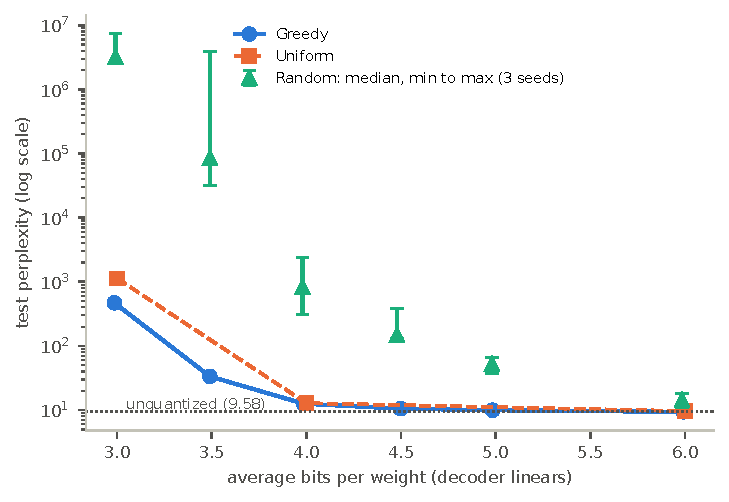
\includegraphics[width=0.85\textwidth]{figures/fig3_ppl_vs_bits.pdf}
\caption{Test perplexity against average width. Greedy and uniform are single evaluations. Random points show the median over three seeds, with bars for the minimum and maximum. The dotted line is the unquantized model. The vertical scale is logarithmic.}
\label{fig:ppl}
\end{figure}

\begin{table}[t]
\centering
\caption{Random allocations by seed. Mean bits is the average width over the three seeds.}
\label{tab:random}
\begin{tabular}{rrrrrr}
\toprule
Budget $B$ & mean bits & seed 0 & seed 1 & seed 2 & median \\
\midrule
6 & 5.98 & 11.12 & 14.26 & 17.98 & 14.26 \\
5 & 4.98 & 37.22 & 51.84 & 66.02 & 51.84 \\
4.5 & 4.48 & 148.17 & 378.16 & 130.55 & 148.17 \\
4 & 3.98 & 822.18 & 2,367 & 308.56 & 822.18 \\
3.5 & 3.49 & 31,530 & 3.87 M & 85,170 & 85,170 \\
3 & 2.99 & 3.20 M & 7.33 M & 2.52 M & 3.20 M \\
\bottomrule
\end{tabular}

\end{table}

\subsection{Bit assignments}

Table~\ref{tab:shares} shows how the greedy allocator spends the budget. At 6 bits, 67 percent of weights stay at 6 bits and 17 percent stay at 8 bits. At 3 bits, 23 percent of weights are at 2 bits and 59 percent are at 3 bits. Mixer units keep more bits than MLP units at every budget: at 4 bits, the mixer averages 4.18 bits and the MLP averages 3.88. Figure~\ref{fig:bits} shows the full assignment. Layer 0 mixer stays at 6 bits across all budgets. Layer 31 MLP keeps 8 bits at budget 6 and 4 bits at budget 3.

\begin{table}[t]
\centering
\caption{Greedy bit assignments. Mixer and MLP columns are the average width within each part. The share columns are the fraction of the 3.57 billion weights at each width.}
\label{tab:shares}
\begin{tabular}{rrrrrrrr}
\toprule
Budget $B$ & mixer bits & MLP bits & 2-bit & 3-bit & 4-bit & 6-bit & 8-bit \\
 & & & \multicolumn{5}{c}{share of parameters (\%)} \\
\midrule
6 & 6.19 & 5.88 & 0.0 & 4.0 & 11.7 & 67.1 & 17.2 \\
5 & 5.23 & 4.84 & 0.0 & 5.9 & 44.1 & 47.7 & 2.2 \\
4.5 & 4.98 & 4.22 & 1.2 & 5.9 & 65.0 & 26.7 & 1.2 \\
4 & 4.18 & 3.88 & 5.1 & 12.7 & 71.5 & 10.7 & 0.0 \\
3.5 & 3.80 & 3.31 & 16.2 & 25.3 & 55.1 & 3.4 & 0.0 \\
3 & 3.18 & 2.88 & 22.6 & 58.7 & 17.6 & 1.2 & 0.0 \\
\bottomrule
\end{tabular}

\end{table}

\begin{figure}[t]
\centering
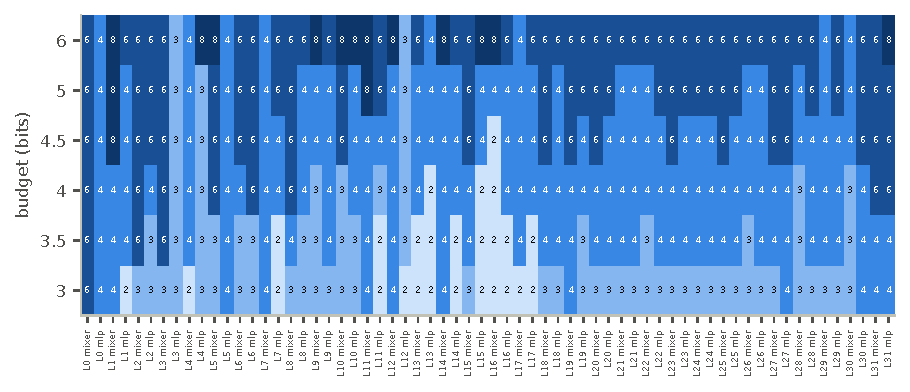
\includegraphics[width=\textwidth]{figures/fig4_greedy_bits.pdf}
\caption{Greedy width for each unit (columns, ordered as in Figure~\ref{fig:heatmap}) at each budget (rows). The number in each cell is the assigned width.}
\label{fig:bits}
\end{figure}

The greedy rule can select steps whose measured cost is negative. A downgrade with negative cost lowers the measured perplexity, so the rule applies it first. On the path to the final allocation, 28 units at budget 6 pass through at least one such step, with 33 steps in total. At budget 3 the count rises to 41 units and 55 steps. These steps are measurement noise rather than real gains, so part of each greedy allocation reflects noise in the sensitivity table.

\subsection{Predictor}

Figure~\ref{fig:pred} compares the additive prediction with the measured sensitivity perplexity. Ranking is preserved well: the Spearman correlation over the 29 unique configurations is 0.96. Magnitude is not preserved. Greedy's measured perplexity exceeds its prediction by factors of 1.04, 1.05, 1.10, 1.26, 3.08, and 32.7 at budgets 6, 5, 4.5, 4, 3.5, and 3. Uniform 4-bit falls within 4 percent of its prediction, whereas uniform 3-bit is 54 times its prediction. Random allocations sit close to the diagonal at 6 bits and far above it at low budgets.

The discrepancy most likely reflects non-additivity. The additive model assumes that quantizing one unit does not change the damage done by quantizing another. That assumption is plausible when each unit contributes a small perturbation. A likely explanation is that errors compound through the residual stream once many units are at 3 or 2 bits. We did not test this mechanism directly. The predictor is therefore reliable for choosing among allocations at moderate budgets and unreliable as an estimate of absolute perplexity below 4 bits.

\begin{figure}[t]
\centering
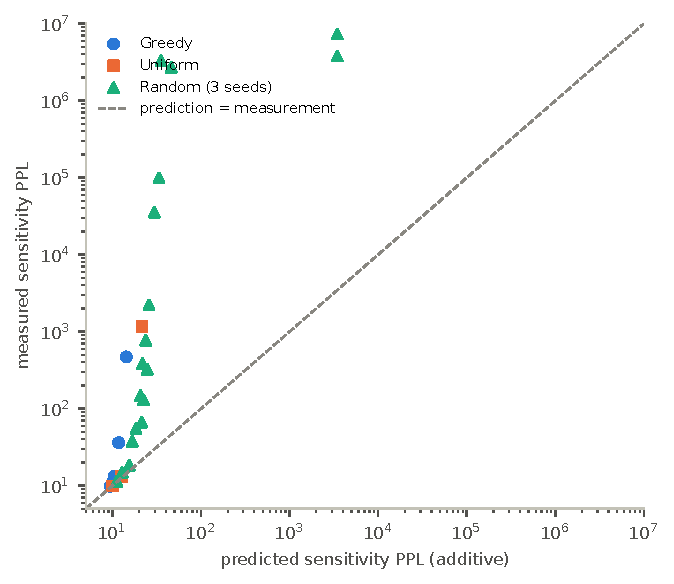
\includegraphics[width=0.7\textwidth]{figures/fig5_pred_vs_measured.pdf}
\caption{Predicted against measured sensitivity perplexity on a logarithmic scale. Each point is one unique configuration. The dashed line marks equality. Points above the line are underpredicted.}
\label{fig:pred}
\end{figure}

\section{Limitations}

First, the sensitivity measurements are noisy. They use 16 windows of 2048 tokens. The 8-bit changes span $-0.016$ to $0.020$, and 41 of 64 units show a fall in measured cost at lower widths. Effects near 4 bits, where the median cost is 0.03, are of similar size to this noise. The ordering of units within a width is less reliable than the ordering between widths.

Second, the additive model underpredicts perplexity at low budgets, by a factor of 33 at 3 bits for the greedy allocation. Conclusions about absolute quality below 4 bits rest on the measured allocations, not the predictor.

Third, every quantity is measured once. We have no repeated runs of the allocation, and the random baseline uses three seeds. The reported differences are single-run comparisons and carry no confidence intervals. The unquantized baseline reproduced to six decimal places in every evaluation in the log, across two separate processes. This supports the determinism of the forward pass but does not estimate the variance of the allocation results.

Fourth, the quantizer is simple. It is round-to-nearest with a symmetric absmax scale per output row. It is not group-wise, activation-aware, or error-compensating, so these results describe that quantizer and should not be read as a statement about GPTQ- or AWQ-style methods.

Fifth, the average widths cover only the decoder linear weights. Embeddings, the output head, and normalization layers, which make up 15.1 percent of the parameters, stay in full precision. The effective size of a deployed model is therefore larger than the average width suggests. The bit counts also use the nominal convention: a 3-bit grid has seven levels, not eight.

Sixth, the perplexity is computed on non-overlapping windows with no context carried across them. Absolute values are therefore higher than values from strided evaluation and should not be compared with published numbers without the same protocol.

Seventh, the evaluation measures language modeling on one corpus. It does not measure task accuracy, and a lower perplexity may not mean better performance on reasoning or mathematics.

Eighth, the run record has gaps. The allocation log comes from a run that found the sensitivity grid already complete, so this log does not record the grid's own timing. Duplicate uniform rows at three budgets came from the allocation code used for the run, and we removed them from every table and figure. Logged non-monotone counts read 64 of 64, but the check in the code tests the wrong direction. From the same table, the correct count is 41 of 64, and only that corrected count appears here.

\section{Conclusion and future work}

In conclusion, the sensitivity table shows a clear structure. One early mixer layer is far more fragile than the rest, MLP units are somewhat more sensitive than mixer units, and the cost of quantization rises steeply below 4 bits. Among allocations that stay within the budget, greedy beats uniform at every budget. The gain is about 2 percent at 6 and 4 bits, and larger at fractional budgets and at 3 bits, where both methods are unusable. Greedy is also far better than random assignment at every budget below 6 bits. Uniform allocations that exceed the budget can outperform greedy, so any comparison must hold the average width fixed. The additive model is useful for ranking but not for estimating absolute perplexity at low widths.

Future work follows from the limitations. The most useful next step is to repeat the sensitivity grid with more windows and several seeds, so that the noise floor is known and the greedy steps with negative cost can be filtered. Pairwise measurements, for example of adjacent layers, would test whether the additive assumption fails in a predictable way. A group-wise quantizer would show whether the sensitivity pattern survives a stronger baseline. Finally, evaluating the selected allocations on task benchmarks would tell us whether perplexity is the right criterion for allocation.

\section*{Reproducibility}

The experiment runs with \texttt{uv run python main.py} from the repository root, and all hyperparameters are in \texttt{config.yaml}. This report is generated from the files in \texttt{results/} by \texttt{python report/make\_report.py}, which writes the figures and tables used here. We checked each number in the text against the script's output.

\begin{thebibliography}{9}
\bibitem{merity2016}
S. Merity, C. Xiong, J. Bradbury, and R. Socher.
\newblock Pointer sentinel mixture models. 2016.

\bibitem{gptq}
E. Frantar, S. Ashkboos, T. Hoefler, and D. Alistarh.
\newblock GPTQ: Accurate post-training quantization for generative pre-trained transformers. 2022.

\bibitem{awq}
J. Lin, J. Tang, H. Tang, S. Yang, et al.
\newblock AWQ: Activation-aware weight quantization for LLM compression and acceleration. 2023.

\bibitem{qwen}
Qwen Team.
\newblock Qwen3.5-4B model card. Hugging Face, \url{https://huggingface.co/Qwen/Qwen3.5-4B}.
\end{thebibliography}

\end{document}
